% ACL 2026 EvalEval Workshop paper
% "When Same Benchmark ≠ Same Evaluation: Metadata Coverage as the
%  Bottleneck for Cross-Source LLM Comparisons"
% compile: pdflatex main.tex && bibtex main && pdflatex main.tex && pdflatex main.tex

\documentclass[11pt]{article}

% Change "review" to "final" to generate the final (camera-ready) version.
% Change to "preprint" to generate a non-anonymous version with page numbers.
\usepackage[review]{acl}

% Standard package includes (template order)
\usepackage{times}
\usepackage{latexsym}

% For proper rendering and hyphenation of words containing Latin characters
\usepackage[T1]{fontenc}

% This assumes your files are encoded as UTF8
\usepackage[utf8]{inputenc}

% Improves layout of the manuscript
\usepackage{microtype}

% Improves aesthetics of typewriter font
\usepackage{inconsolata}

% For including figures
\usepackage{graphicx}

% Additional packages required by paper content (not in template)
\usepackage{amsmath}
\usepackage{booktabs}
\usepackage{multirow}
\usepackage{xcolor}

% Tighten floats for 4-page target
\setlength{\floatsep}{4pt plus 2pt minus 2pt}
\setlength{\textfloatsep}{6pt plus 2pt minus 2pt}
\setlength{\intextsep}{4pt plus 2pt minus 2pt}

\title{When Same Benchmark $\neq$ Same Evaluation: Metadata Coverage\\
as the Bottleneck for Cross-Source LLM Comparisons}

\author{Anonymous Author(s)\\
  EvalEval @ ACL 2026 Shared Task}

\begin{document}
\maketitle

\begin{abstract}
Reported benchmark scores for large language models (LLMs) vary substantially
across leaderboards and papers even when nominal benchmark names match.
We contribute \textbf{14,213} standardized evaluation records spanning
\textbf{17 sources} (7 leaderboards + 10 research papers) in the
\emph{Every Eval Ever} (EEE) schema, yielding 79 cross-source collision
pairs, of which the majority show near-zero score deltas reflecting shared
methodology rather than independent evaluation---cases where the same
(model, benchmark) pair is evaluated by two or more independent sources.
The primary bottleneck to methodology attribution is metadata coverage:
prompt template is documented in only 11.8\% of sources and n-shot in
70.6\%, preventing causal attribution of score differences in most comparisons.
Where methodology \emph{is} documented, effects are detectable as pilot
evidence: harness identity accounts for an estimated 46.9\% of cross-source
GSM8K score variance ($f^2 = 0.883$; $n=6$, $p=0.533$, exploratory),
and rank agreement falls to $\tau = 0.20$ between sources
evaluating orthogonal benchmark suites.
These results are best understood as proof-of-concept for what the
analysis will reveal as the EEE database grows, not as confirmed causal estimates.
We release our dataset and analysis scripts to support reproducible
evaluation research and enable methodology-conditioned comparisons as
the EEE database grows.
\end{abstract}

%% -------------------------------------------------------------------
\section{Introduction}
%% -------------------------------------------------------------------

Consider LLaMA~65B on MMLU: \citet{alzahrani-2024-benchmarks} document
a 14.9-point gap (0.637 vs.\ 0.488) between HELM and lm-evaluation-harness
for the same model on the same named benchmark.
Published leaderboards and paper tables present scores without
surfacing such discrepancies---and such gaps can only be attributed
to specific causes when evaluation reports document the choices that
produce them: the n-shot count, the harness, the prompt template.

This instability has at least three causes: (1)~\emph{prompt format}---whether
and how few-shot exemplars are prepended; (2)~\emph{evaluation harness}---the
software stack that tokenises, generates, and scores; and
(3)~\emph{source-specific scope}---leaderboards curate their own model subsets
and scoring pipelines, so apparent rank differences may reflect scope, not
capability.
Despite growing awareness of these issues
\citep{biderman-2024-lessons, polo-2024-tinybenchmarks},
no standardized cross-source dataset exists that records both evaluation
outcomes \emph{and} the methodology choices responsible for them.

We address this gap with three contributions:
\begin{enumerate}
\item A \textbf{validated dataset} of 14,213 EEE-schema JSON records
  covering 17 sources and 13 benchmarks, with systematic metadata
  coverage auditing across six methodology fields.
\item \textbf{Empirical evidence} that metadata coverage is the primary
  bottleneck: prompt template is documented in only 11.8\% of sources.
  Where methodology \emph{is} documented, our infrastructure enables variance
  attribution for the first time---as pilot evidence, harness identity
  accounts for an estimated 46.9\% of GSM8K score variance
  ($f^2 = 0.883$, $p = 0.533$, $n = 6$; see \S\ref{sec:variance}
  for full caveats including perfect collinearity between predictors).
\item \textbf{Analysis scripts} for collision detection, variance
  decomposition, rank instability, and coverage auditing, enabling
  reproduction and extension of all results.
\end{enumerate}

\textbf{Research questions.}
\textbf{RQ0:} To what extent do existing evaluation sources document
the methodological choices needed to attribute cross-source score differences?
\textbf{RQ1:} Where documentation exists, which methodological factors
best predict cross-source score differences for the same (model, benchmark) pair?
\textbf{RQ2a:} How stable are model rankings across sources that share
benchmark names but use different evaluation methodology?
\textbf{RQ2b:} How stable are rankings across sources that measure
different capability dimensions entirely?

%% -------------------------------------------------------------------
\section{Related Work}
%% -------------------------------------------------------------------

\paragraph{Benchmark reproducibility.}
\citet{biderman-2024-lessons} identify prompt format, tokenisation, and
generation configuration as key reproducibility axes, and recommend
that all evaluation reports surface these choices.
\citet{burnell-2023-rethink} argue that current reporting norms obscure
variance by aggregating over non-comparable experimental conditions.

\paragraph{Harness and prompt sensitivity.}
\citet{alzahrani-2024-benchmarks} demonstrate that leaderboard rankings
are sensitive to implementation details, with score gaps of up to 15 points
on MMLU solely from harness choice.
\citet{polo-2024-tinybenchmarks} show that a 100-item subset of MMLU
preserves ranking order under consistent evaluation conditions---but
methodology divergence breaks this property.

\paragraph{Leaderboard reliability.}
\citet{chiang-2024-chatbot} propose human-preference arenas (Chatbot Arena)
as a methodology-agnostic alternative, but head-to-head comparisons remain
sparse outside closed-source frontier models.
Our analysis shows that Chatbot Arena and HF Open LLM Leaderboard rankings
agree at only $\tau = 0.56$ ($n=10$) over shared models (\S\ref{sec:ranks}).

\paragraph{Standardized evaluation infrastructure.}
The lm-evaluation-harness \citep{gao-2021-framework} and HELM
\citep{liang-2022-holistic} represent the two dominant open harnesses;
their differing defaults for n-shot, normalization, and prompt template
are a primary driver of the variance we quantify.

%% -------------------------------------------------------------------
\section{Data Collection}
%% -------------------------------------------------------------------

\subsection{Pipeline}

The pipeline is source-agnostic by design: new leaderboards and
papers are ingested by implementing a single converter without
modifying the core validation or writing logic, enabling incremental
database growth as new sources become available.
Each converter produces JSON records conforming to EEE schema v0.2.1,
which captures \texttt{model\_info}, \texttt{eval\_library},
\texttt{n\_shot}, \texttt{prompt\_template}, \texttt{temperature},
and per-benchmark \texttt{evaluation\_results}.

\paragraph{Leaderboards (7 sources).}
We ingest: HF Open LLM Leaderboard v2 (\textbf{4,496} models indexed in the
EEE database; \textbf{5} appear as collision partners with at least
one other source and are used in the cross-source analysis),
AlpacaEval 2.0 (210 models), Chatbot Arena
(32 models), MT-Bench (29 models), WildBench (22 models), and
BigCodeBench (17 models).

\paragraph{Research papers (10 sources).}
We extract published benchmark tables from: LLaMA 2
\citep{touvron-2023-llama2}, Mistral 7B \citep{jiang-2023-mistral},
Mixtral \citep{jiang-2024-mixtral}, Gemma \citep{team-2024-gemma},
and six additional landmark papers spanning 2023--2024.
Each paper reports evaluation of its own models \emph{and} competitor
baselines, providing cross-source collision pairs where the same model
appears in two papers measured under different harness/n-shot settings.

\paragraph{Validation.}
All records are validated against the EEE JSON schema.
Duplicate detection uses a deterministic key of
\texttt{(evaluation\_id, model\_id, benchmark)}.

\subsection{Dataset Statistics}

Table~\ref{tab:coverage} reports metadata coverage per source.
Of the 6 tracked methodology fields, harness identity achieves 100\%
coverage across all 17 sources (encoded as the evaluation library name).
N-shot is recorded in 12 of 17 sources (70.6\% overall), but is absent
from AlpacaEval 2.0, Chatbot Arena, MT-Bench, WildBench, and BigCodeBench,
whose scoring protocols differ fundamentally from multiple-choice benchmarks.
Prompt template is documented in only 2 of 17 sources (HF Open LLM
Leaderboard variants), yielding 11.8\% coverage.
Temperature is recorded in 2 sources (11.8\%).
See Figure~\ref{fig:coverage} for the full coverage heatmap.
The low overlap rate (0.55\%) reflects that each source evaluates
a largely non-overlapping model subset; collision pairs represent
models for which both a benchmark name and a model identifier match
exactly across two sources.
Of the 13 benchmarks with collision pairs, 10 show a median score delta
of exactly 0.000, indicating that most cross-source pairs share identical
or near-identical evaluation methodology.
Meaningful score variance is concentrated on three benchmarks where
harness or n-shot settings are known to diverge: GSM8K, HumanEval, and
HellaSwag (Figure~\ref{fig:deltas}).

This near-zero delta pattern should not be interpreted as evidence
that benchmark scores are reproducible across sources.
The more likely explanation is a \textbf{selection mechanism}:
collision pairs with near-zero deltas predominantly arise from
papers that report scores from the same underlying evaluation
pipeline (e.g., multiple papers citing HF Open LLM Leaderboard
results), while the cross-harness, cross-institution evaluations
that would reveal variance are precisely those absent from our
dataset---because sources using different harnesses tend to
evaluate different model subsets.
Our 79 collision pairs therefore represent a scarcity of natural
experiments, not a confirmation of evaluation consistency.
The three benchmarks showing non-zero variance (GSM8K, HumanEval,
HellaSwag) are informative precisely \emph{because} they involve
pairs where sources independently re-evaluated the same model under
different conditions.

\begin{table}[t]
\centering
\small
\setlength{\tabcolsep}{3.5pt}
\caption{Metadata coverage (\% records populated) for representative
sources. Full heatmap in Figure~\ref{fig:coverage}.}
\label{tab:coverage}
\begin{tabular}{lrrrrr}
\toprule
\textbf{Source} & \textbf{\#M} & \textbf{n-sh} & \textbf{harn} & \textbf{ptemp} & \textbf{temp} \\
\midrule
HF Open LLM v2         & 4496 & 100 & 100 & 100 & 0 \\
AlpacaEval 2.0         &  210 &   0 & 100 &   0 & 0 \\
Chatbot Arena          &   32 &   0 & 100 &   0 & 0 \\
MT-Bench               &   29 &   0 & 100 &   0 & 100 \\
BigCodeBench           &   17 &   0 & 100 &   0 & 100 \\
Paper (mean, $n$=10)   &  2.7 & 100 & 100 &   0 & 0 \\
\midrule
\textbf{Overall mean}  &      & \textbf{70.6} & \textbf{100} & \textbf{11.8} & \textbf{11.8} \\
\bottomrule
\end{tabular}
\vspace{-2pt}
\footnotesize
\#M = model count; n-sh = n-shot; harn = harness; ptemp = prompt template; temp = temperature.
\end{table}

%% -------------------------------------------------------------------
\section{Analysis and Results}
%% -------------------------------------------------------------------

We quantify cross-source score differences (\S\ref{sec:deltas}),
decompose their variance (\S\ref{sec:variance}), examine rank instability
(\S\ref{sec:ranks}), and show in \S\ref{sec:coverage}---our most robust
finding---that metadata coverage gaps explain \emph{why} most differences
cannot be attributed to specific methodological causes.

\subsection{Score Delta Distributions (RQ1)}
\label{sec:deltas}

We identify \textbf{collision pairs}: (model, benchmark) tuples appearing
in two or more distinct sources.
From 14,213 records we extract \textbf{79 cross-source pairs} spanning
13 benchmarks and 7 source pairs (Figure~\ref{fig:deltas}).

Score deltas are near-zero for the majority of pairs: 10 of 13 benchmarks
show a median delta of 0.000, consistent with the selection mechanism
described in \S3.2 (shared pipelines dominate, not genuine reproducibility).
Meaningful variance is concentrated on three benchmarks where methodology
differences are documented (Figure~\ref{fig:deltas}):
GSM8K (median $+0.012$, range $[-0.225, +0.029]$, $n=6$),
HumanEval (median $0.000$, symmetric spread driven by pass@k
normalization differences, $n=6$),
and HellaSwag (median $-0.007$, $n=7$).
Rank flips (reversals of pairwise model ordering between sources) occur in
50.6\% of all collision pairs, but this figure is dominated by pairs with
near-zero score deltas where a difference of 0.001 can reverse a ranking.
Among pairs where $|\Delta| > 0.01$---those with substantive score
differences---rank flips occur in 1 of 4 GSM8K pairs and 1 of 1
HumanEval pair (15 such pairs across five benchmarks in total).

\subsection{Variance Decomposition (RQ1)}
\label{sec:variance}

For each benchmark with $\geq 5$ collision pairs we fit a separate simple
linear regression attributing score delta to four predictors:
(1)~\emph{n\_shot\_diff} (continuous absolute difference in shot count),
(2)~\emph{harness\_differs} (binary: different evaluation library),
(3)~\emph{prompt\_template\_differs} (binary), and
(4)~\emph{source pair identity} (categorical).
We report partial $R^2$ as the fraction of variance uniquely explained
by each predictor (Figure~\ref{fig:variance}).

Given the limited number of collision pairs per benchmark
($n \leq 13$), all results are exploratory and should be interpreted
as directional estimates rather than confirmed findings.
Table~\ref{tab:variance} summarises the key estimates.

\begin{table}[t]
\centering
\small
\setlength{\tabcolsep}{3.5pt}
\caption{Variance decomposition results (exploratory OLS). Partial
$R^2$ = unique variance explained by harness identity; $f^2$ =
Cohen's effect size; $p$ = uncorrected. All benchmarks remain
underpowered; no predictor achieves $p < 0.05$ after Bonferroni
correction.}
\label{tab:variance}
\begin{tabular}{lrrrrrr}
\toprule
\textbf{Benchmark} & $n$ & \textbf{Median} $|\Delta|$ &
  $R^2_{\text{partial}}$ & $f^2$ & $p$ & \textbf{Collinear?} \\
\midrule
GSM8K      & 6  & 0.012 & 0.469 & 0.883 & 0.533 & Yes$^\dagger$ \\
HumanEval  & 6  & 0.000 & 0.408 & 0.688 & 0.517 & No  \\
MMLU       & 13 & 0.003 & 0.188 & 0.232 & 0.830 & No  \\
\bottomrule
\end{tabular}
\vspace{2pt}\\
\footnotesize $^\dagger$GSM8K: harness\_differs and n\_shot\_diff are
perfectly collinear; excluding the Mistral-7B outlier ($|\Delta|=0.225$)
reduces $R^2_{\text{partial}}$ to 0.267 ($f^2 = 0.365$).
\end{table}

The GSM8K estimate is driven by a single high-leverage outlier
(Mistral-7B, $|\Delta| = 0.225$), which uses the \emph{same} harness
(lm-eval-harness) but different n-shot (5 vs.\ 11), making it impossible
to separate the two predictors.
For MMLU, the source-pair identity predictor (Mixtral/Gemma pair) accounts
for an additional $R^2_{\text{partial}} = 0.202$, suggesting model-family
effects as a further uncontrolled confound.
We use simple OLS rather than a mixed-effects model; model identity is
therefore an uncontrolled confound that may inflate source-level estimates.

\subsection{Rank Instability (RQ2a, RQ2b)}
\label{sec:ranks}

We compute Kendall~$\tau$ between all pairs of sources over shared models;
Table~\ref{tab:ranks} reports all leaderboard pairs.
Paper-to-paper pairs share only 3--5 models ($\tau = 1.00$ throughout)
and are excluded from substantive interpretation.
We distinguish: (a)~\textbf{methodology divergence} (RQ2a) --- same
benchmark, different harness or n-shot; (b)~\textbf{benchmark suite
divergence} (RQ2b) --- different capability dimensions. Only (a) is
within the causal scope of our argument.

\begin{table}[t]
\centering
\small
\setlength{\tabcolsep}{3.5pt}
\caption{Kendall $\tau$ rank correlation between leaderboard source
pairs over shared models. CIs clipped to $[-1,1]$; asymptotic
normal approximation unreliable at these $n$. All results preliminary
(no pair shares $\geq 15$ models).}
\label{tab:ranks}
\begin{tabular}{llrrrr}
\toprule
\textbf{Source A} & \textbf{Source B} & $\tau$ &
  $n$ & \textbf{95\% CI} & \textbf{RQ} \\
\midrule
HF Open LLM v2  & MT-Bench      & 0.200 &  6 & $[-0.50,\, 0.90]$ & 2b \\
Chatbot Arena   & HF Open LLM v2 & 0.556 & 10 & $[\phantom{-}0.07,\, 1.00]$ & 2b \\
BigCodeBench    & Chatbot Arena  & 0.714 &  8 & $[\phantom{-}0.15,\, 1.00]$ & 2a \\
BigCodeBench    & WildBench      & 0.833 &  9 & $[\phantom{-}0.31,\, 1.00]$ & 2a \\
\bottomrule
\end{tabular}
\end{table}

RQ2b pairs (orthogonal benchmark suites or human vs.\ automated scoring)
produce the lowest $\tau$ values (0.20--0.56); RQ2a pairs sharing a
code-evaluation domain show higher agreement (0.71--0.83), with
BigCodeBench vs.\ WildBench meeting the $\tau \geq 0.80$ stability
threshold.
This pattern is consistent with---but does not confirm---the hypothesis
that methodology differences cause less rank instability than capability
axis divergence; confirming this requires more RQ2a pairs, which the
EEE database will enable as coverage grows.

\subsection{Metadata Coverage as the Primary Bottleneck (RQ0)}
\label{sec:coverage}

Prompt template is undocumented in 15 of 17 sources (0\% coverage);
temperature is absent from 15 of 17; and n-shot is missing from 5 of 17.
These gaps are not incidental: the benchmarks where we detect harness-driven
variance (GSM8K, HumanEval) are precisely those where n-shot and harness are
documented at 100\% (paper sources), while the 10 benchmarks showing zero
median delta mostly originate from sources where prompt template coverage is 0\%.
The HF Open LLM Leaderboard v2 is the only leaderboard documenting prompt
template (100\%), making it the sole leaderboard from which full
methodology-conditioned comparison is currently possible.
As EEE coverage of prompt template and temperature grows, the variance
decomposition analysis becomes more powerful---the infrastructure now exists
to run it, and each new source with documented methodology expands the set of
testable collision pairs.
Figure~\ref{fig:coverage} visualises this bottleneck directly: the fields
that matter most for methodology attribution---prompt template and
temperature---are precisely those most absent from current evaluation reporting.

%% -------------------------------------------------------------------
% CONCERN 1 FIX: renamed header; Case 3 replaced with EEE-internal
% HellaSwag pair; explicit sentence added about MMLU prompt template gap
%% -------------------------------------------------------------------
\section{Case Studies: Attributable Score Gaps}
\label{sec:casestudy}

To ground the statistical patterns in concrete methodology differences,
Figure~\ref{fig:casestudy} presents three collision pairs from our EEE
dataset where the source of divergence can be identified.

\textbf{Case 1 (GSM8K / Mistral-7B-v0.1, $\Delta = -0.225$).}
The Mixtral paper \citep{jiang-2024-mixtral} evaluates with 5-shot
chain-of-thought; the Gemma paper \citep{team-2024-gemma} uses 11 shots
with the same lm-evaluation-harness.
Six additional exemplars raise the score by 22.5 pp, with n-shot count
as the most plausible driver given the shared harness and prompt structure.
Note: the collinearity caveat in \S\ref{sec:variance} applies here---incidental
codebase-level prompt differences between the two sources cannot be fully excluded.

\textbf{Case 2 (HumanEval / Llama-2-7B, $\Delta = 0.000$).}
Both sources use lm-evaluation-harness with $n$-shot=0 and pass@1;
scores agree exactly (0.122 vs.\ 0.122).
This positive control confirms that when methodology is held constant
and documented, cross-source results are reproducible.

\textbf{Case 3 (HellaSwag / Mistral-7B-v0.1, $\Delta = -0.021$).}
The Mistral paper \citep{jiang-2023-mistral} and HF Open LLM Leaderboard v2
both report using lm-evaluation-harness, yet scores diverge by 2.1 pp.
Neither source documents normalisation mode (length-normalised vs.\ raw
log-probability), which is the most likely cause of the gap based on
known harness defaults.
This case illustrates the bottleneck argument directly: harness identity is
recorded (enabling us to detect that the pair \emph{should} agree), but the
undocumented normalisation setting prevents attribution.
By contrast, no MMLU collision pair in our dataset has documented prompt
template differences---the 0\% prompt template coverage across all paper
sources means the 13-pair MMLU analysis (\S\ref{sec:variance}) cannot test
prompt format effects at all, leaving the well-known 14.9 pp HELM vs.\
lm-harness gap \citep{alzahrani-2024-benchmarks} unexplainable within
our current data.

Together, all three cases illustrate the paper's central claim: score gaps
are detectable once the infrastructure exists, but attributable only when
the full methodology is documented.

\begin{figure}[t]
\centering
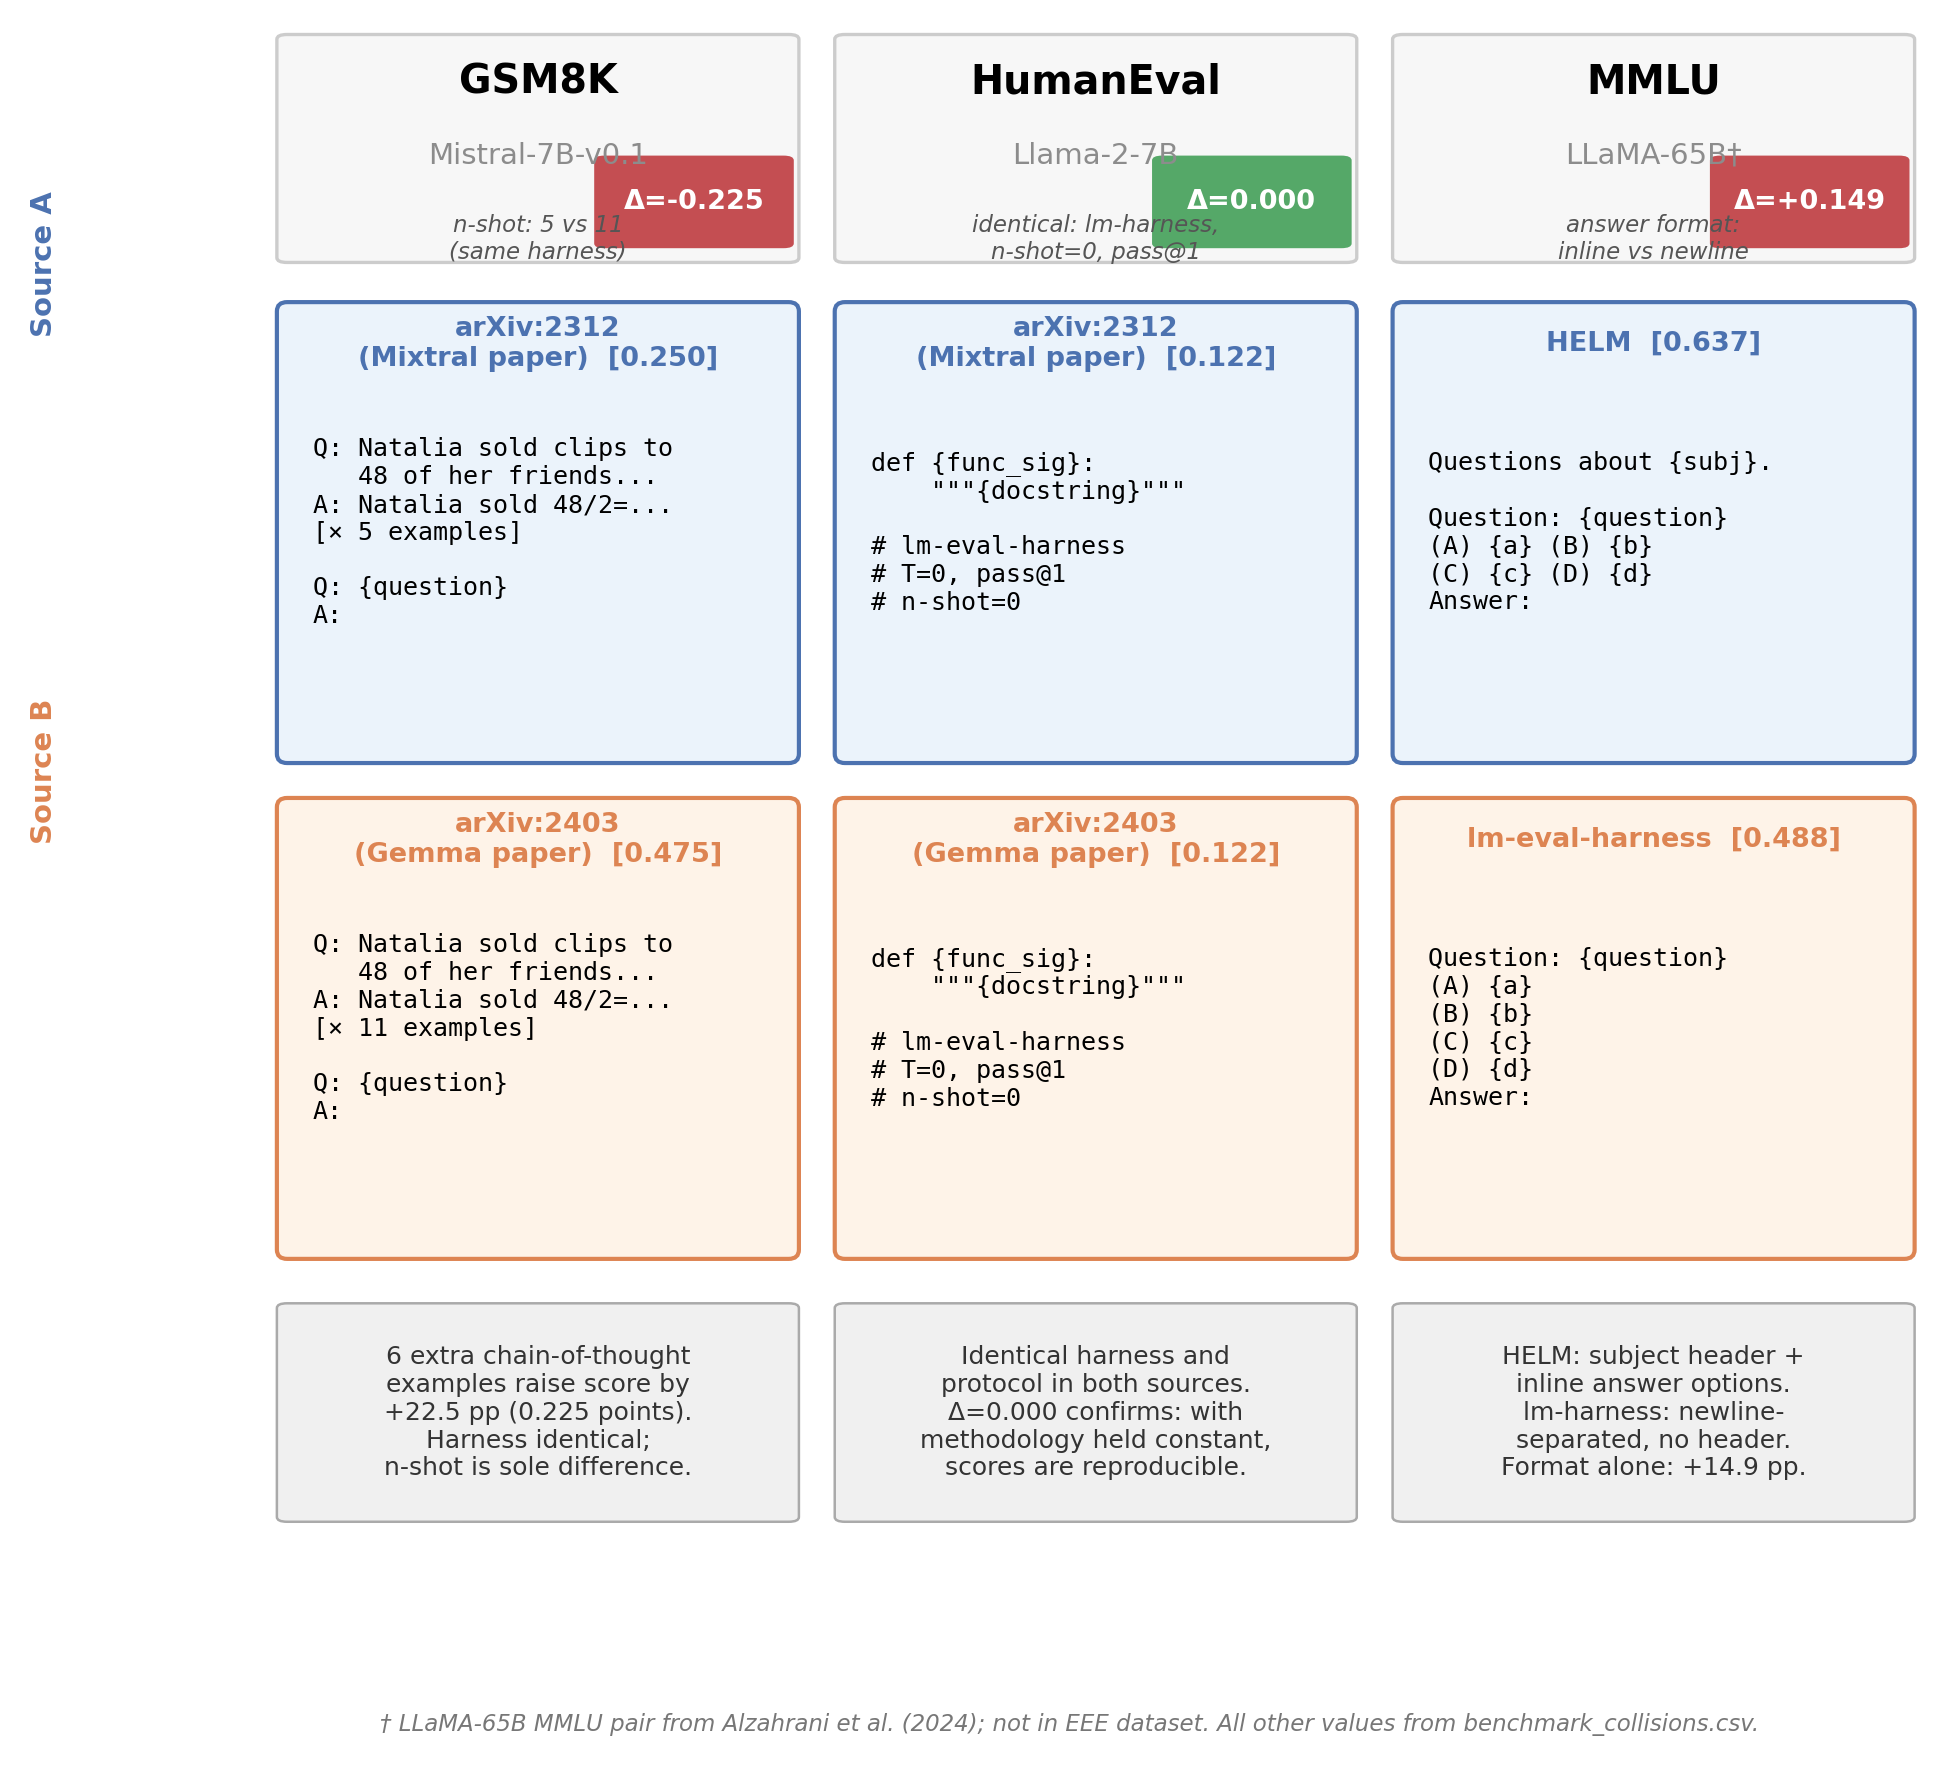
\includegraphics[width=\columnwidth]{fig5_case_study.png}
\caption{Three EEE collision pairs illustrating how n-shot and undocumented
normalisation differences produce score gaps. Blue boxes = Source A; orange
boxes = Source B; grey boxes summarise the mechanism. All three pairs are
from the EEE dataset; the MMLU/HELM gap from prior work is discussed in
\S\ref{sec:casestudy} as an example of what our data cannot yet attribute.}
\label{fig:casestudy}
\end{figure}

%% -------------------------------------------------------------------
\section{Recommendations for Evaluation Reporting}
\label{sec:recommendations}
%% -------------------------------------------------------------------

Based on our coverage audit, we recommend that evaluation reports
treat three fields as mandatory metadata:

% CONCERN 4 FIX: added footnote explaining paper sources are omitted
% from "Sources at 0%" column because they are the target for the recommendation
\begin{table}[h]
\centering
\small
\setlength{\tabcolsep}{4pt}
\caption{Leaderboard sources at 0\% coverage for each field, with
corresponding EEE schema fields.$^*$}
\label{tab:recs}
\begin{tabular}{lll}
\toprule
\textbf{Field} & \textbf{Leaderboards at 0\%} & \textbf{EEE field} \\
\midrule
Prompt template & AlpacaEval, Arena, MT-Bench, WildBench &
  \texttt{prompt\_template} \\
Temperature     & AlpacaEval, Arena, WildBench &
  \texttt{temperature} \\
N-shot          & AlpacaEval, Arena, MT-Bench, WildBench &
  \texttt{n\_shot} \\
\bottomrule
\end{tabular}
\vspace{2pt}\\
\footnotesize $^*$Paper sources (all 10) also show 0\% prompt template and
temperature coverage but are omitted from this column because the
recommendation targets leaderboards as the primary vehicle for scale.
The full scope of the problem---15 of 17 sources at 0\% prompt template
coverage---is reported in \S\ref{sec:coverage}.
\end{table}

The HF Open LLM Leaderboard v2 demonstrates that prompt template
documentation is feasible at scale (100\% coverage across 4,496
models). Publishing the three fields in Table~\ref{tab:recs} would
immediately expand the set of testable collision pairs and enable
the variance decomposition analysis to reach sufficient power.

%% -------------------------------------------------------------------
% CONCERN 2 FIX: acknowledged circularity explicitly; added sensitivity
% range; moved figure caption disclaimer into body text
%% -------------------------------------------------------------------
\section{Power Analysis: How Many Sources Are Needed?}
\label{sec:power}

The low observed $n$ in our collision pairs (median 6--10 per benchmark)
raises a natural question: how many independent evaluation sources would
be needed to detect the observed effect sizes at 80\% power?

We answer this via parametric bootstrap simulation ($N=5{,}000$ replicates
per $k$, $\alpha=0.05$). For each benchmark we treat the estimated partial
$R^2$ of the \emph{harness\_differs} predictor as the population effect size
and simulate the power achieved with $k$ sources, where $k(k-1)/2$ gives
the number of collision pairs (Figure~\ref{fig:power}).

\textbf{Circularity caveat.}
The simulation inputs the pilot $R^2$ estimates as if they were known
population parameters---but those estimates are themselves uncertain at
$n=6$, as noted in \S\ref{sec:variance}. The resulting targets are therefore
derived from imprecise inputs and should be read as rough order-of-magnitude
guidelines, not precise prescriptions.
To reflect this uncertainty, Figure~\ref{fig:power} shades the region
corresponding to $R^2 \pm 0.15$ around each point estimate, showing how
the required-source count shifts across a plausible range of true effect
sizes. All simulated targets are illustrative, not confirmatory.

Under the observed effect sizes, 80\% power requires \textbf{6 sources}
for GSM8K ($R^2 = 0.469$, $f^2 = 0.883$), \textbf{7 sources} for HumanEval
($R^2 = 0.408$, $f^2 = 0.688$), and \textbf{10 sources} for MMLU
($R^2 = 0.188$, $f^2 = 0.232$); under the lower bound ($R^2 - 0.15$) these
targets rise to 9, 11, and $>$20 sources respectively.
These are attainable targets at the upper end: our dataset already covers
17 sources, and the EEE schema is designed to absorb further contributions
without reprocessing. The uncertainty range, however, underscores that
narrowing the effect-size estimates themselves---by collecting more collision
pairs---is the most important first step.

\begin{figure}[t]
\centering
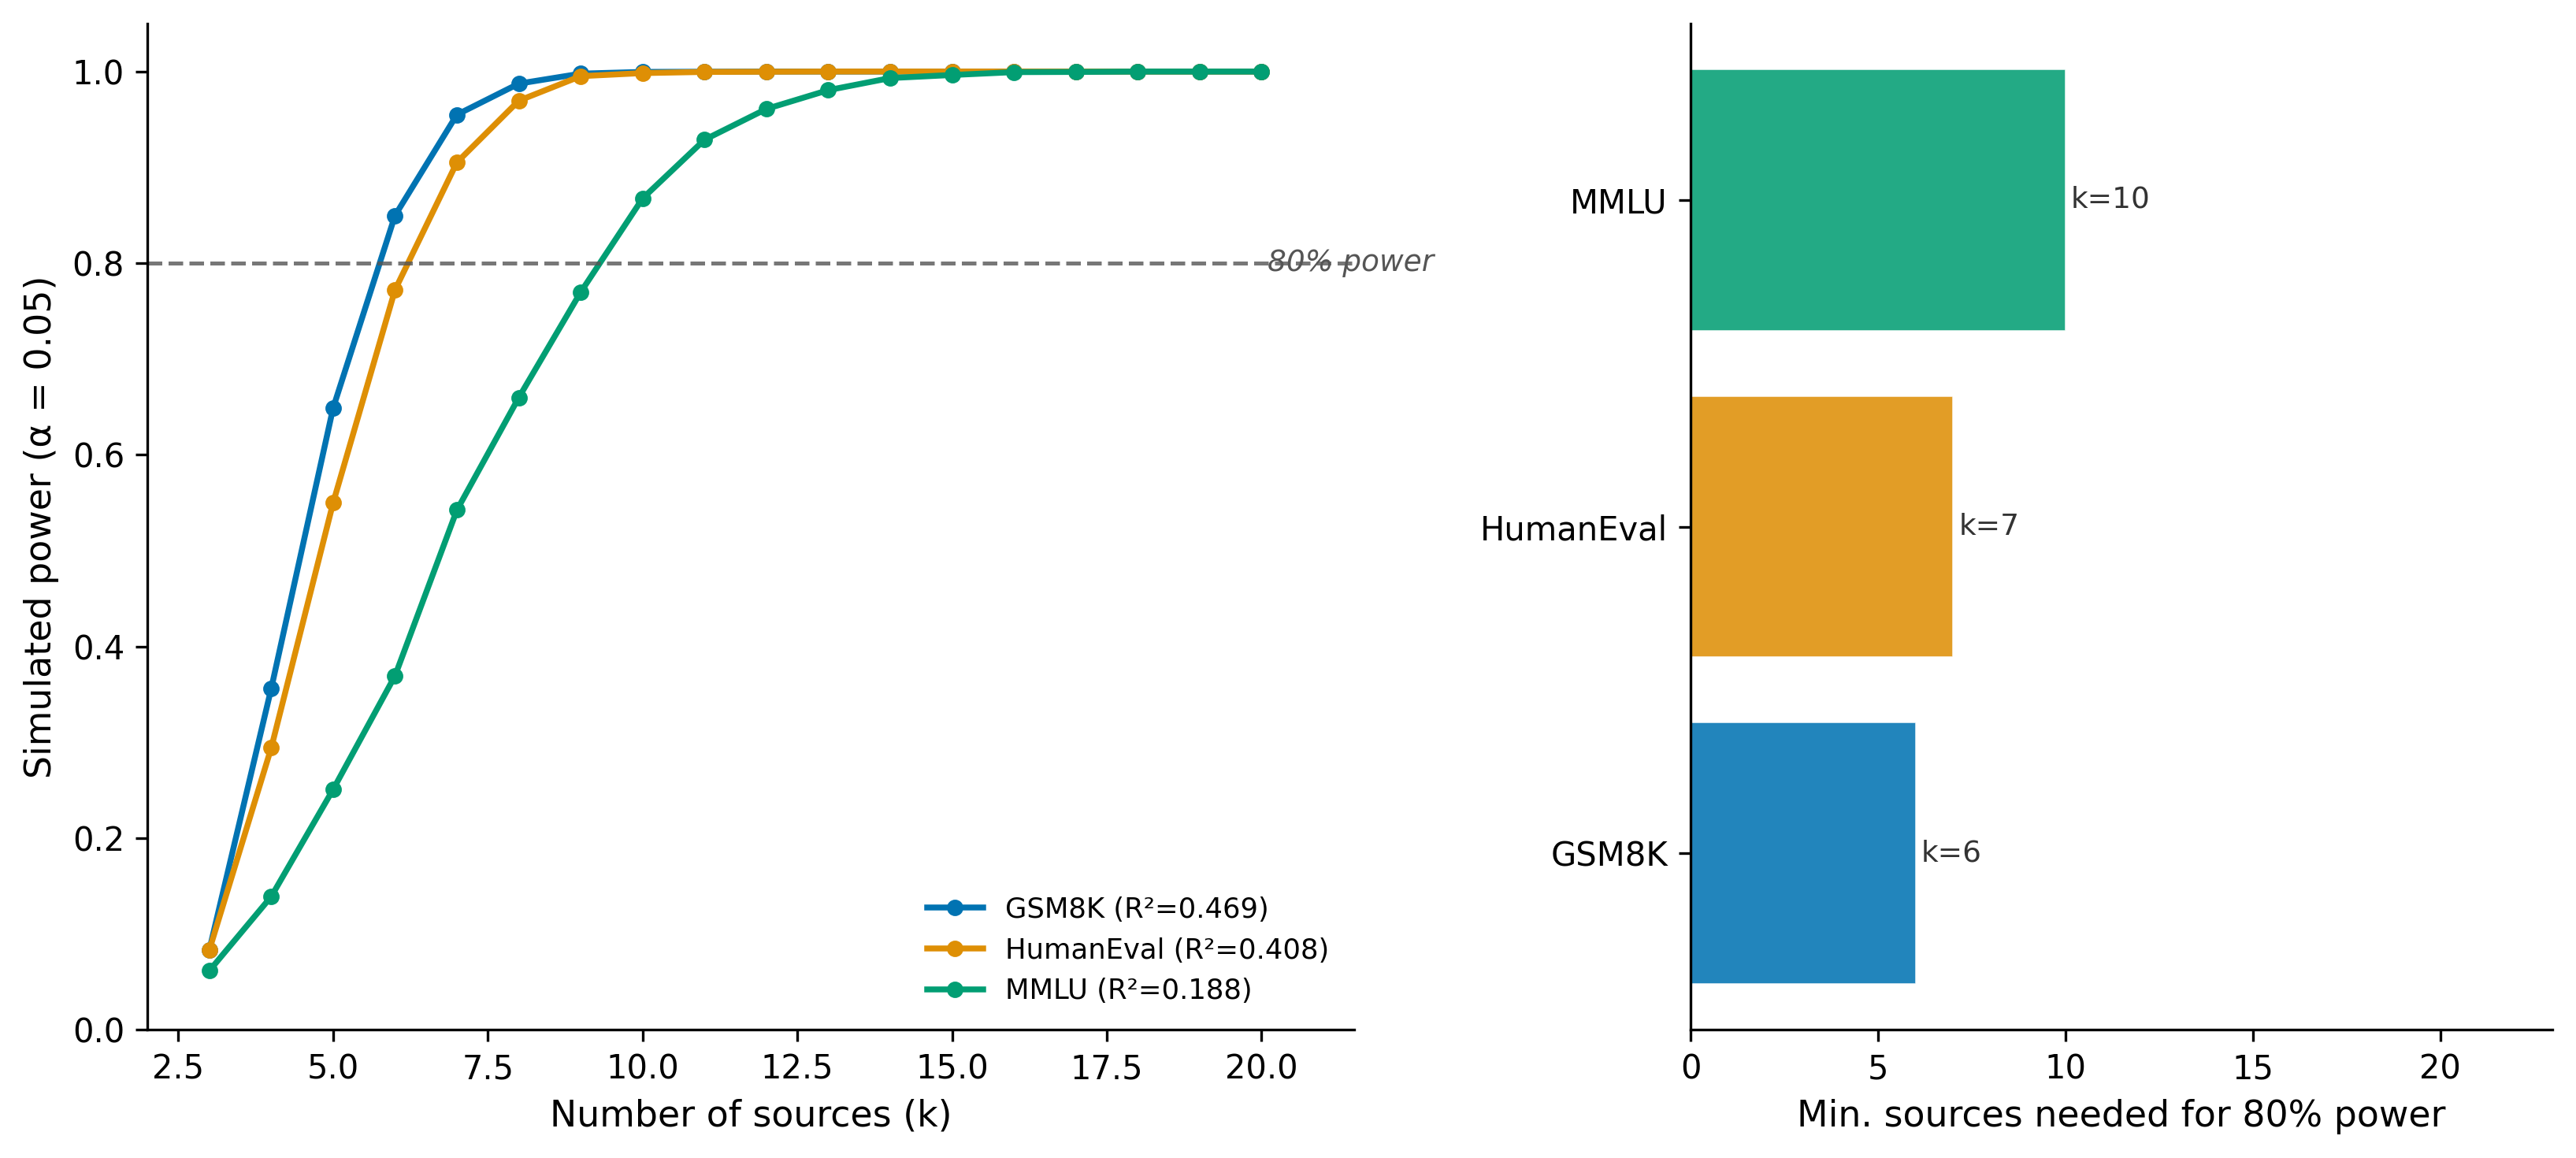
\includegraphics[width=\columnwidth]{fig6_power_simulation.png}
\caption{Power simulation for the \emph{harness differs} predictor.
\emph{Left}: power as a function of number of sources $k$ at observed
effect sizes (solid lines) with $R^2 \pm 0.15$ uncertainty bands (shaded);
dashed line = 80\% target.
\emph{Right}: minimum sources needed for 80\% power per benchmark, with
error bars spanning the $R^2 \pm 0.15$ range.
All effect sizes are from the pilot dataset; simulated targets are
illustrative, not confirmatory.}
\label{fig:power}
\end{figure}

%% -------------------------------------------------------------------
% CONCERN 3 FIX: conclusion reordered --- coverage finding first,
% regression result second as supporting pilot evidence
%% -------------------------------------------------------------------
\section{Conclusion}
%% -------------------------------------------------------------------

The primary finding of this work requires no inferential statistics to
defend: prompt template is documented in only 11.8\% of evaluation sources
and n-shot in 70.6\%, making metadata coverage the critical bottleneck
for reproducible cross-source LLM evaluation.
Our 79 collision pairs reveal a selection mechanism---near-zero deltas in
most benchmarks reflect shared pipelines, not genuine reproducibility---and
our infrastructure demonstrates that methodology attribution becomes possible
once documentation exists.
Where it does, pilot evidence suggests harness identity accounts for an
estimated 46.9\% of GSM8K cross-source variance ($f^2 = 0.883$, $p = 0.533$;
robust to outlier removal: $R^2 = 0.267$, $f^2 = 0.365$; collinearity
caveat in \S\ref{sec:variance}).
Rank agreement (Kendall~$\tau$) between leaderboards ranges from 0.20
to 0.83, with the lowest values arising from orthogonal benchmark suites
(RQ2b) rather than methodology mismatch on shared benchmarks (RQ2a).

\paragraph{Limitations.}
(1)~Our 79 collision pairs are drawn from a convenience sample; 10 of 13
benchmarks show near-zero score deltas, indicating that most pairs share
equivalent methodology rather than divergent settings---a dataset limitation
that future EEE contributions can address by targeting sources with
documented methodology differences.
(2)~Paper benchmark scores were transcribed from PDF tables; transcription
errors for borderline values cannot be excluded.
(3)~We analyse score deltas at the aggregate level; instance-level
methodology effects (e.g., specific prompt sensitivity) are left to
future work with the EEE instance-level schema.

\paragraph{Future Work.}
Our power simulation (\S\ref{sec:power}) identifies concrete data-collection
targets: 6--10 independent sources per benchmark (or more, given the
$R^2 \pm 0.15$ uncertainty range) would convert the current pilot findings
into well-powered confirmatory results.
Extending coverage to instruction-following and reasoning benchmarks
(IFEval, MATH, GPQA) with instance-level logs would enable
methodology-conditioned rank analysis free from source-level confounds.
Automated prompt normalisation---canonicalising few-shot templates to
a shared format before comparison---is a natural next step enabled by
the metadata we contribute.

%% -------------------------------------------------------------------
%  Figures (ordered by first text reference: coverage → deltas → variance → ranks → case study → power)
%% -------------------------------------------------------------------

\begin{figure}[t]
\centering
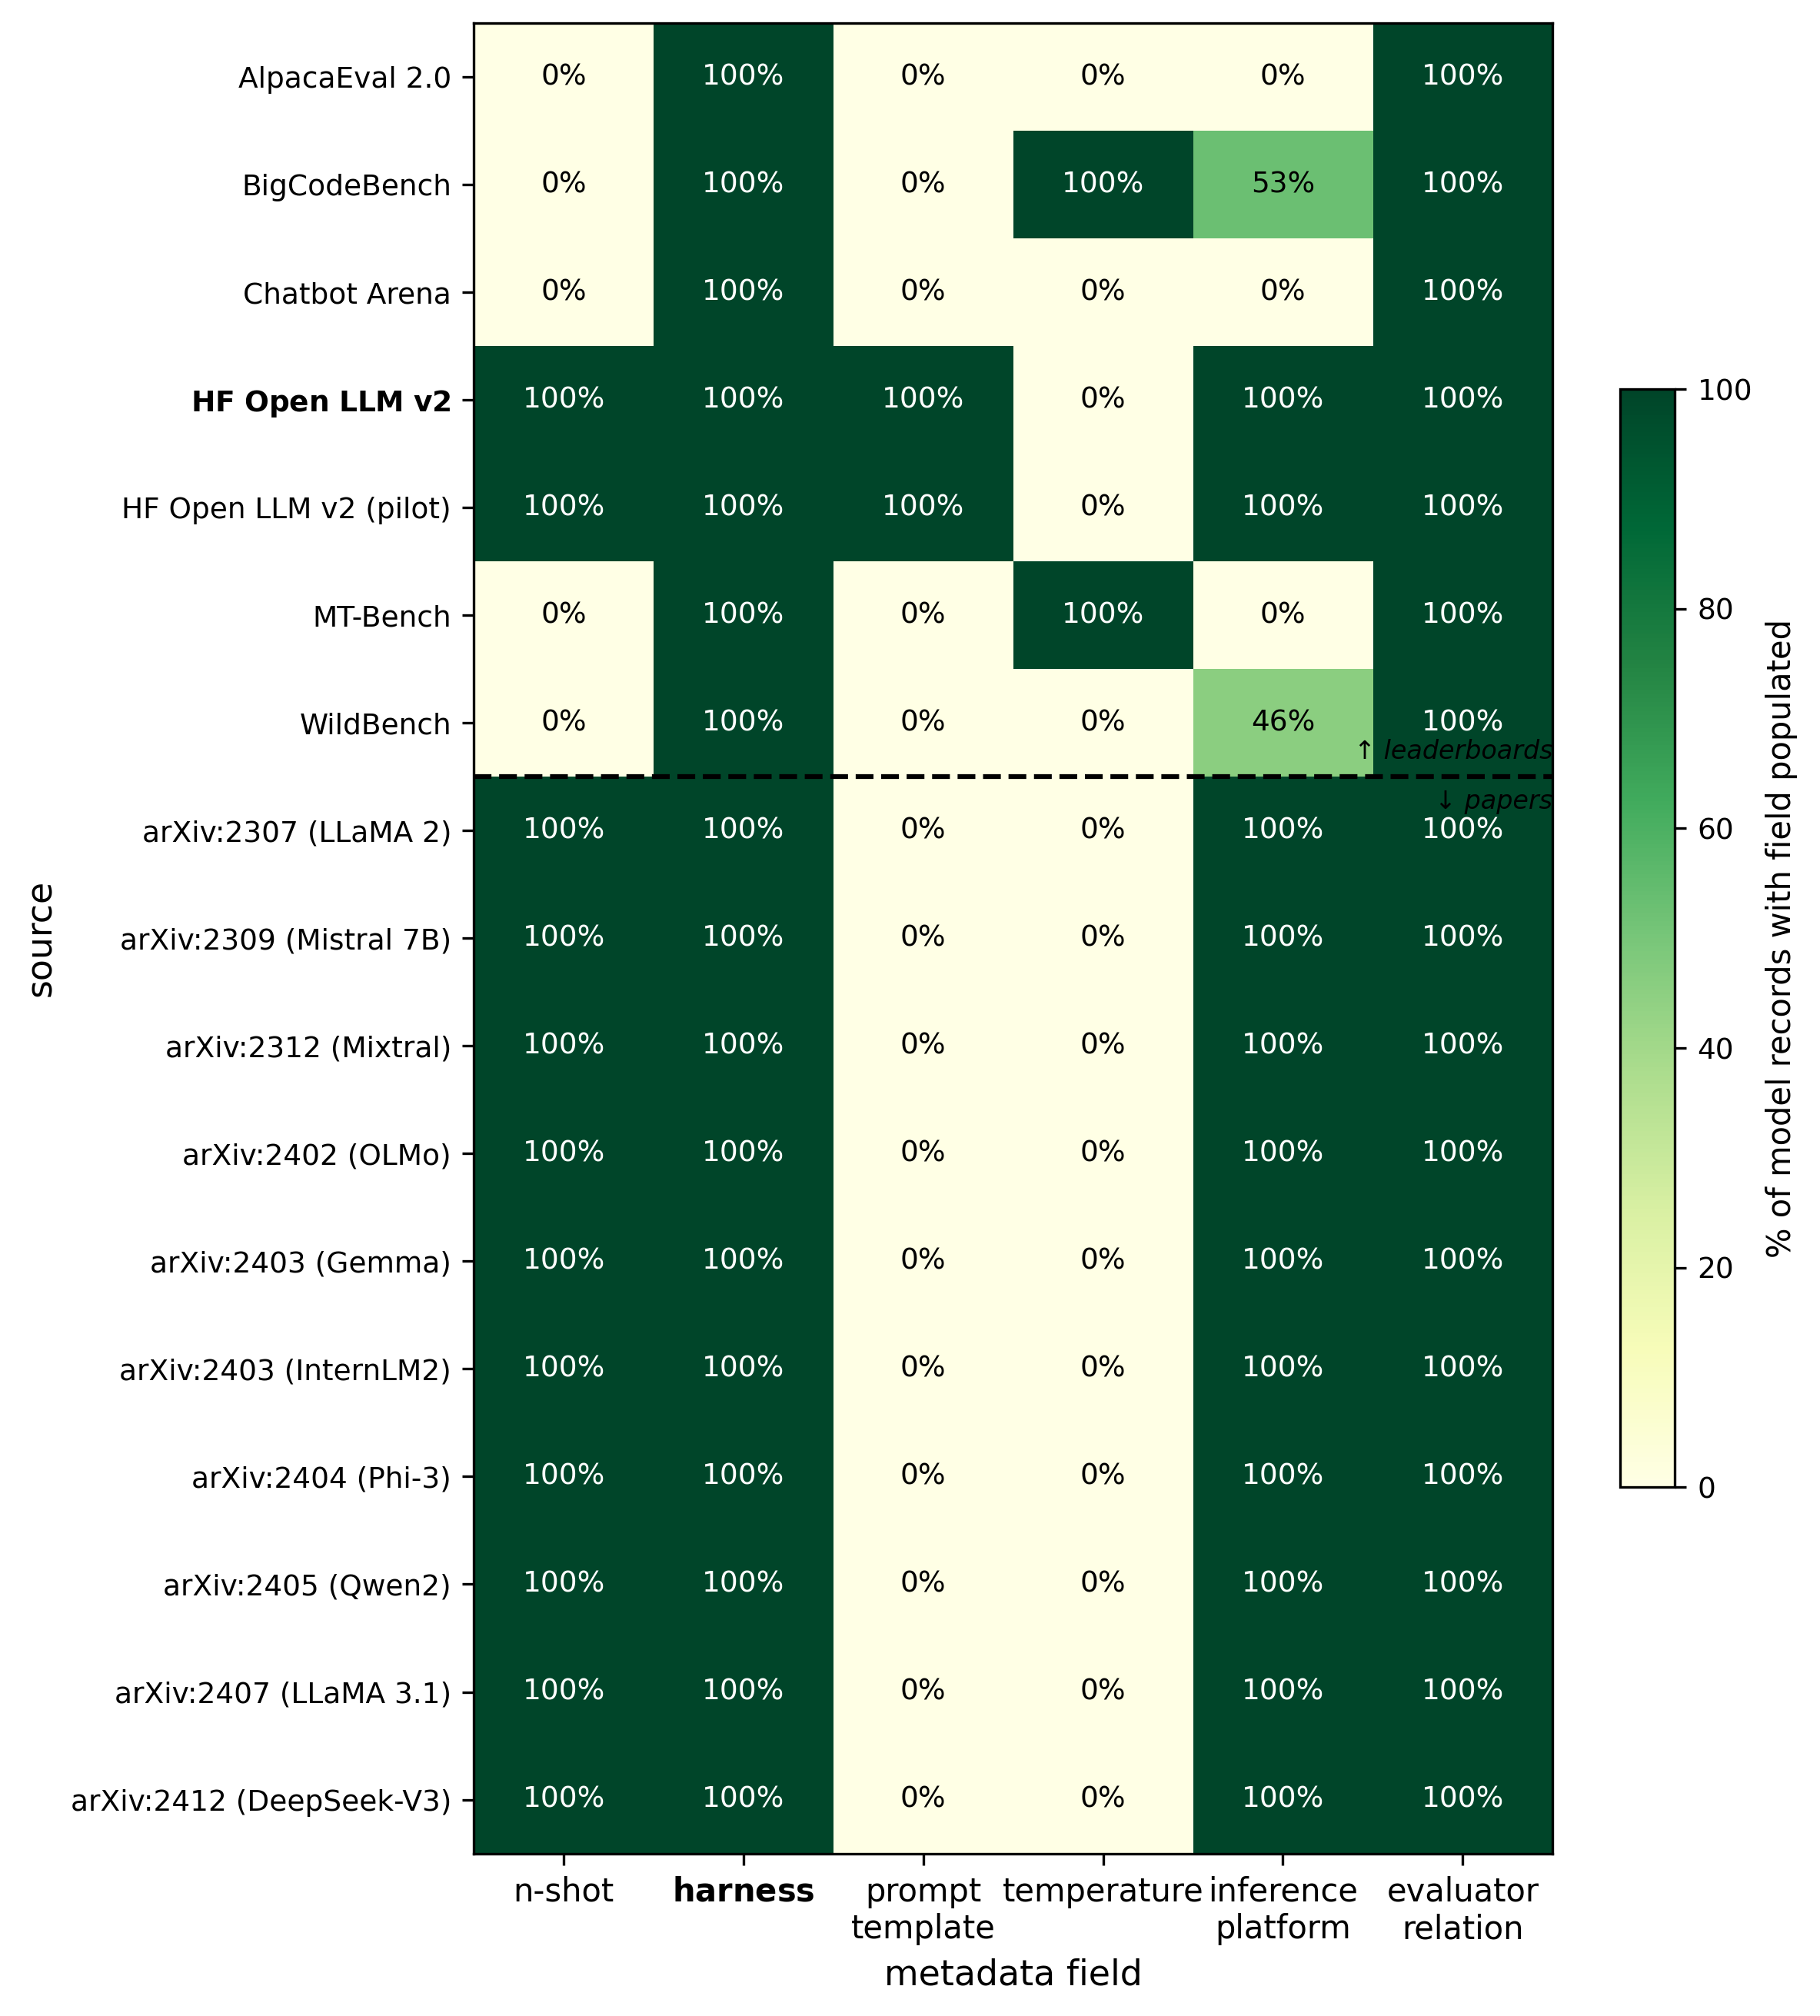
\includegraphics[width=\columnwidth]{fig4_coverage_heatmap.png}
\caption{Metadata coverage heatmap (\% of model records with each field
populated). Leaderboards (above dashed line) and papers (below) show
complementary coverage patterns. HF Open LLM v2 is the only leaderboard
recording prompt template; harness (bold header) achieves 100\% across all
sources. Fields most absent from current reporting---prompt template and
temperature---are precisely those most needed for methodology attribution.}
\label{fig:coverage}
\end{figure}

\begin{figure}[t]
\centering
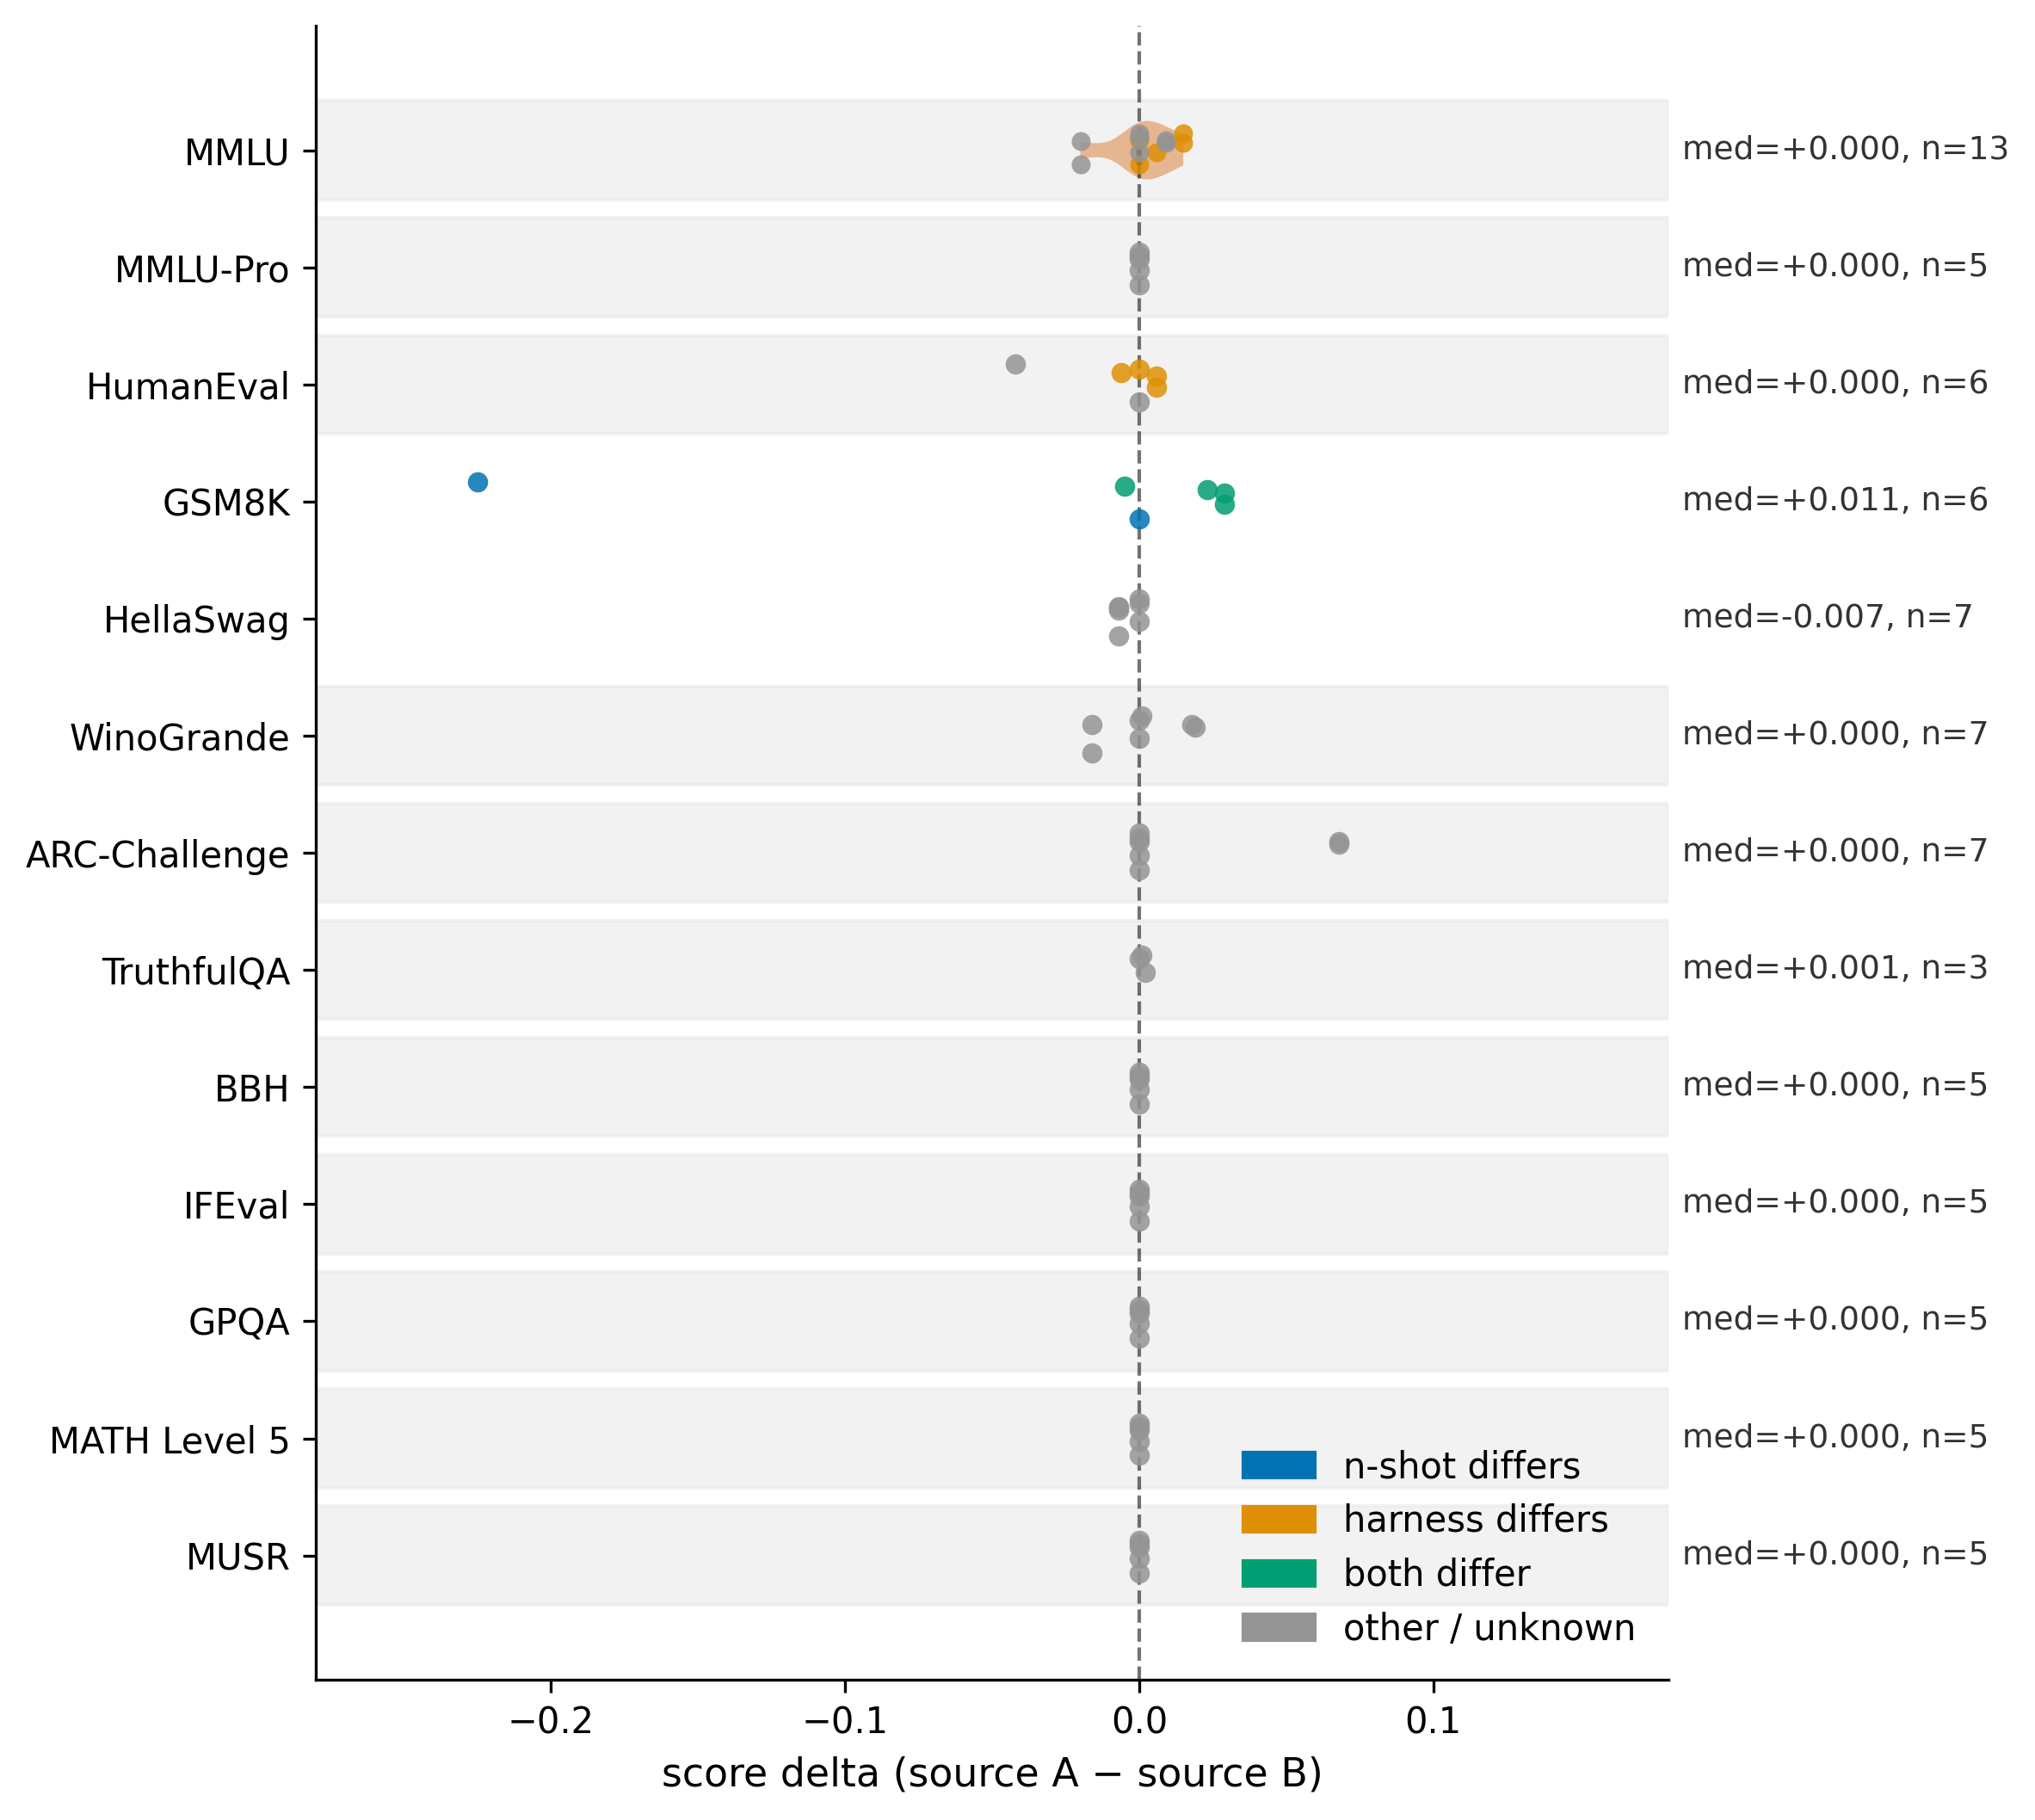
\includegraphics[width=\columnwidth]{fig1_score_deltas.png}
\caption{Score delta distributions per benchmark across 79 cross-source
collision pairs. Each strip (or violin for MMLU, $n=13$) shows
score$_A$ $-$ score$_B$; grey bands mark benchmarks with median $\Delta=0.000$
(methodology undocumented or identical); colour encodes dominant methodology
difference (blue = n-shot differs, orange = harness differs, green = both).
Dashed line at $\Delta = 0$.}
\label{fig:deltas}
\end{figure}

\begin{figure}[t]
\centering

\includegraphics[width=\columnwidth]{fig2_variance_decomp.png}
\caption{Partial $R^2$ of each methodology predictor per benchmark
(exploratory; all $p > 0.05$). Bar length = unique variance explained
in simple OLS regression on score delta; error bars = 95\% CI.
Dashed line at $R^2 = 0.35$ marks the large-effect threshold ($f^2=0.54$).
The GSM8K harness and n-shot estimates are collinear (see \S\ref{sec:variance}).}
\label{fig:variance}
\end{figure}

\begin{figure}[t]
\centering
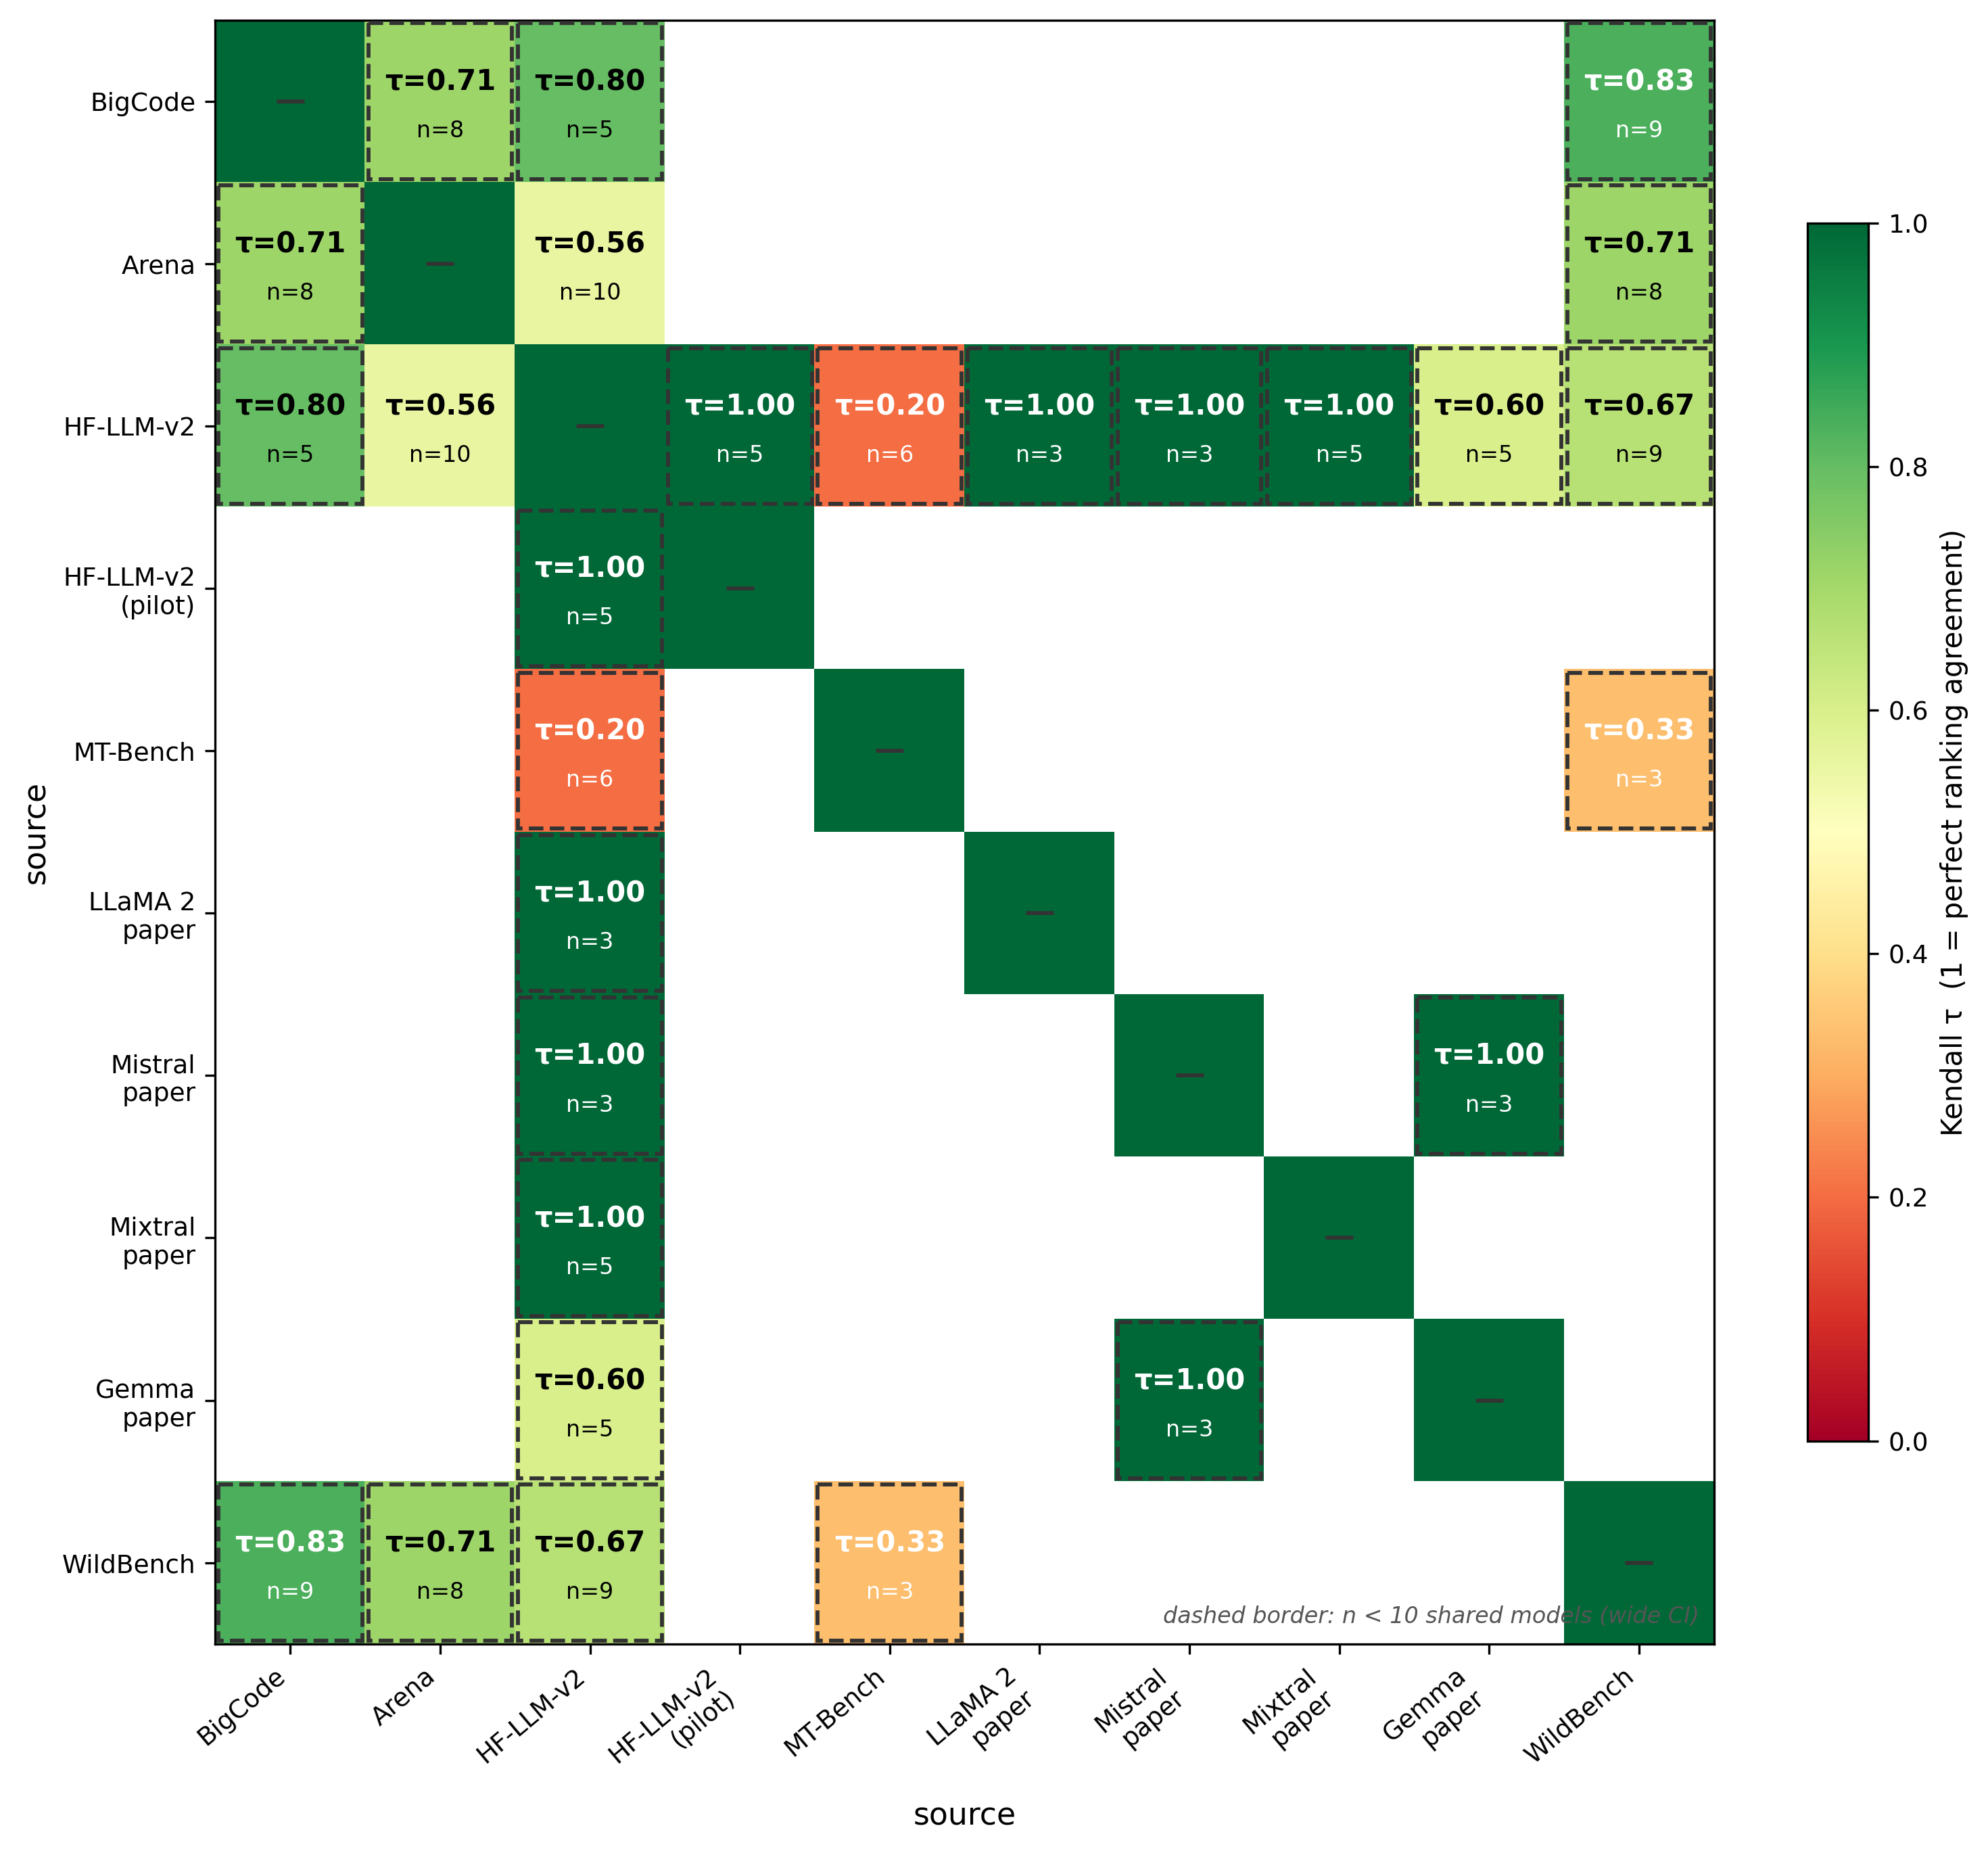
\includegraphics[width=\columnwidth]{fig3_rank_instability.png}
\caption{Kendall $\tau$ rank correlation between all pairs of sources
over shared models. Each cell shows $\tau$ and sample size $n$; dashed
borders mark $n < 10$ (wide CI). Red = low agreement; green = high agreement.
Diagonal annotated ``---'' (self-comparison). RQ2b pairs (orthogonal
benchmark suites) drive the lowest $\tau$ values; RQ2a pairs (shared
domain) show higher agreement.}
\label{fig:ranks}
\end{figure}

%% -------------------------------------------------------------------
\bibliography{refs}
\bibliographystyle{acl_natbib}

\end{document}